
\textit{D'après << Réplique de la mission InSIGHT >>, MP 2019.}

On s'intéresse ici au sous-système SEIS. Il est basé sur un instrument
hybride composé :
\begin{itemize}
\item d'un système de déploiement (DPL);
\item d'une sphère comportant trois capteurs sismiques à très larges bandes et leurs capteurs de
température;%. La sphère dispose d’un système de référencement de ses pieds (figure 3). Sa masse est d'environ \SI{3}{kg};
\item d'une boîte électronique d'acquisition dont la structure est donnée par le diagramme de
définition des blocs. 
\end{itemize}


\begin{figure}[!h]
\centering
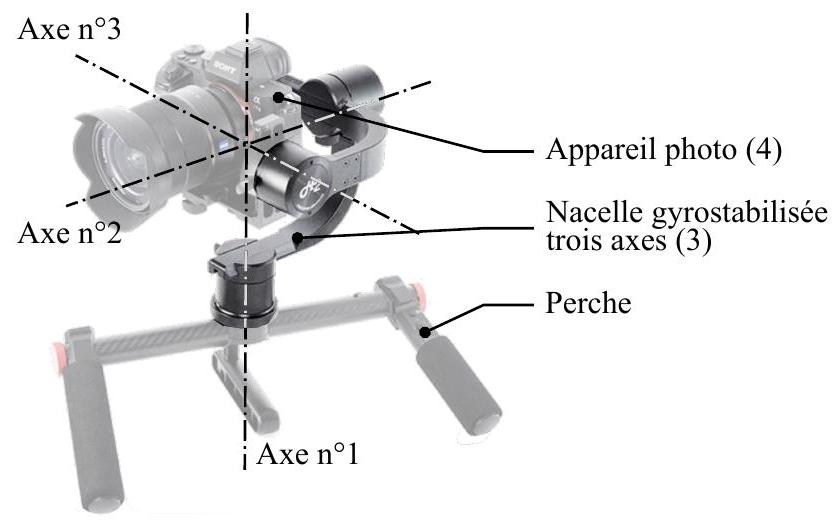
\includegraphics[width=5cm]{fig_01.jpg}
\caption{Sous-système SEIS \label{fig_01}}
\end{figure}

Afin d'être positionné, le SEIS est équipé de 3 pieds positionnés par des vérins électriques(aussi appelés actionneurs linéaires) asservis en position. Leur chaîne structurelle est donnée sur la figure \ref{fig_09}.

\begin{figure}[!h]
\centering
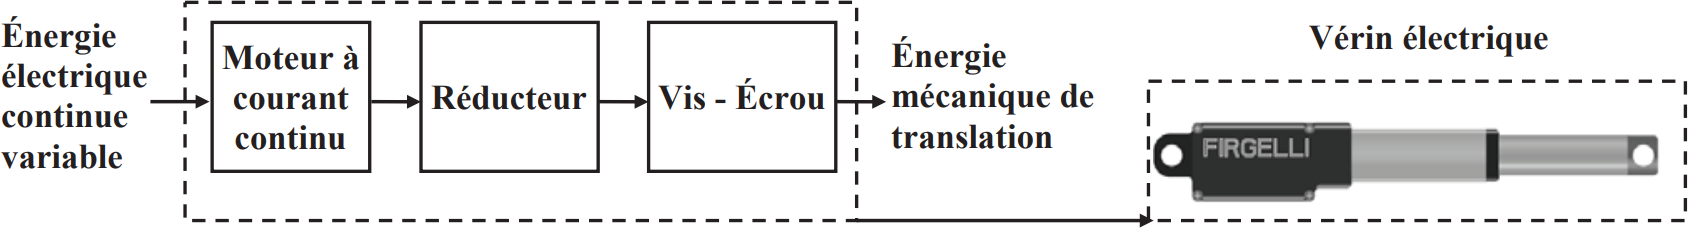
\includegraphics[width=\linewidth]{fig_09.png}
\caption{Chaîne structurelle de l’actionneur électrique linéaire \label{fig_09}}
\end{figure}


\textbf{Notations et spécifications :}
\begin{multicols}{2}
\begin{itemize}
\item masse à déplacer pour chaque vérin : $M =\SI{1}{kg}$;
\item pesanteur de la Terre : $g = \SI{9,81}{m.s^{-2}}$;
\item rapport de réduction du réducteur : $r = 0,01$;
\item rendement du réducteur : $\eta_r = 0,95$;
\item pas de la vis du système vis-écrou : $p = \SI{12}{mm}$;
\item rendement du système vis-écrou : $\eta_v = 0,96$;
\item coefficient de frottement visqueux du moteur : $f=\SI{0,002}{Nms/rad}$;
\item moment d’inertie équivalent total ramené sur l’arbre moteur : $J = \SI{0,00004}{kg.m^2}$;
\item résistance de l’induit de la MCC (Machine à Courant Continu) : $R =\SI{1}{\Omega}$;
\item inductance de l’induit de la MCC : $L = \SI{20}{\mu H}$;
\item constante de couple : $K_c = \SI{0,35}{NmA^{-1}}$;
\item constante de force contre électromotrice : $K_e = \SI{0,35}{Vs/rad}$;
\item tension d’alimentation de l’induit de la MCC : $u(t)$ en \si{V};
\item courant absorbé par l’induit de la MCC : $i(t)$ en \si{A};
\item vitesse de rotation en sortie de la MCC : $\omega(t)$ en \si{rad/s};
\item position angulaire en sortie de la MCC :  $\theta(t)$ en \si{rad};
\item force contre électromotrice de la MCC : $e(t)$ en \si{V};
\item couple moteur de la MCC : $C_m(t)$ en \si{Nm};
\item couple résistant total ramené sur l’arbre moteur : $C_r(t) = \dfrac{Mgpr}{2\pi \eta_v \eta_r} h(t)$\footnote{$h(t)$ désigne la fonction de Heaviside qui prend la valeur 0 pour t<0, 1 sinon.} en \si{Nm}.
\end{itemize}
\end{multicols}

\textbf{Équations du moteur à courant continu :}
\begin{multicols}{2}
\begin{itemize}
\item équation électrique : $u(t)=e(t)+Ri(t)+L\dfrac{\dd i(t)}{\dd t}$;
\item équations de couplage électro-mécanique : $e(t)=K_e \omega(t)$, $C_m(t)=K_C i(t)$.
\end{itemize}
\end{multicols}

\subsection*{Modélisation de la motorisation}

La structure du schéma-bloc obtenue à partir du modèle de connaissance de la MCC est présentée sur la figure suivante.

\begin{figure}[!h]
\centering
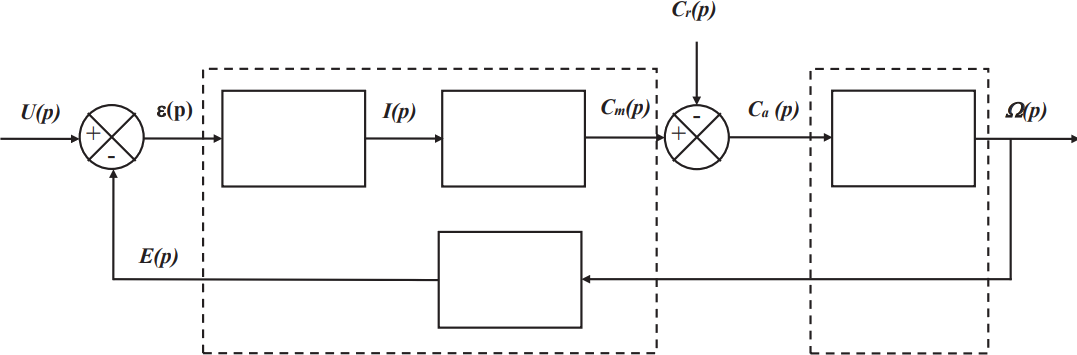
\includegraphics[width=.8\linewidth]{dr_01.png}
\caption{Structure du schéma bloc \label{dr_01}}
\end{figure}

\question{À partir des équations du moteur à courant continu, compléter sous forme
littérale les schémas bloc modélisant la MCC.}

L'application du théorème du moment dynamique à l'arbre moteur permet d'écrire l'équation suivante : 
$$
J\dfrac{\dd \omega(t)}{\dd t}  = C_m(t)-C_r(t)-f\omega(t).
$$

\question{Compléter le schéma-bloc.}

On se place dans le cas particulier où $C_r(p) = 0$.

\question{Donner l’expression, sous sa forme canonique, de la fonction de transfert en boucle fermée $\indice{F}{m1}(p)=\dfrac{\Omega(p)}{U(p)}$.}


La figure \ref{dr_02} présente les résultats expérimentaux de l’évolution de la vitesse de rotation, $\omega(t)$ à la suite de l’application d’un échelon de tension $u(t)$ d’une amplitude de \SI{12}{V} aux bornes de la MCC. On pose $\indice{F}{m2}(p)=\dfrac{\Omega(p)}{U(p)} = \dfrac{F_0}{1+T_0p}$

\begin{figure}[!h]
\centering
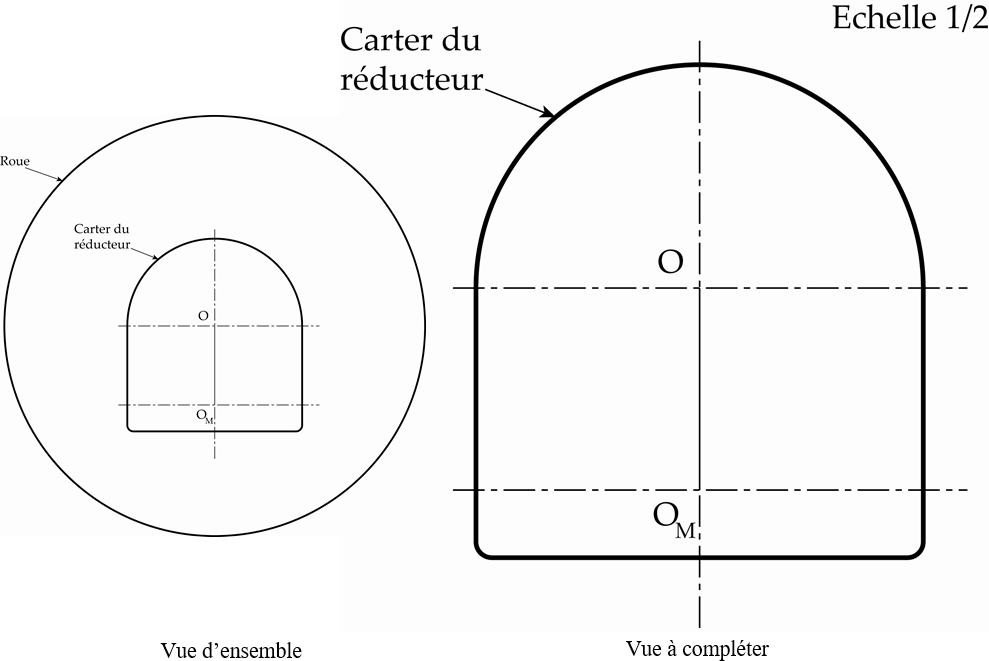
\includegraphics[width=.8\linewidth]{dr_02.png}
\caption{Réponse de la MCC à un échelon de \SI{12}{V}\label{dr_02}}
\end{figure}

% Q18
\question{Justifier le choix d’une fonction de transfert d’ordre 1 pour modéliser le comportement de la MCC à partir des essais expérimentaux. Effectuer les constructions graphiques nécessaires sur 
la figure \ref{dr_02} afin de déterminer la valeur du gain statique $F_0$
et de la constante de temps $T_0$ de $\indice{F}{m2}(p)$. Proposer une hypothèse simplificatrice permettant de justifier le passage à l’ordre 1 de $\indice{F}{m2}(p)$ par rapport à $\indice{F}{m1}(p)$.}


\subsection{Étude de l’asservissement en position du vérin}

\begin{obj}
Choisir un correcteur approprié permettant de satisfaire le cahier des charges vis-à-vis des 
exigences concernant l’asservissement en position du vérin électrique suivant l’axe $\vect{y_0}$
conformément à la figure 11.
\end{obj}

\begin{figure}[!h]
\centering
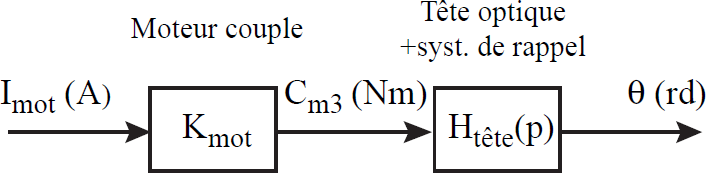
\includegraphics[width=.8\linewidth]{fig_11.png}
\caption{Déplacement de la tige du vérin\label{fig_11}}
\end{figure}

La mesure de la distance est obtenue grâce à un capteur à ultrason permettant de délivrer, sous la 
forme d’impulsions, une image de la distance entre la structure sur SEIS et le sol. Cette information 
est ensuite traitée afin de générer un signal image de la distance parcourue par la tige du vérin.

L’étude précédente a permis d’obtenir un modèle de comportement de la MCC intégré dans le schéma bloc de l’asservissement présenté en figure \ref{fig_12} pour lequel $C_r(p)=0$

\begin{figure}[!h]
\centering
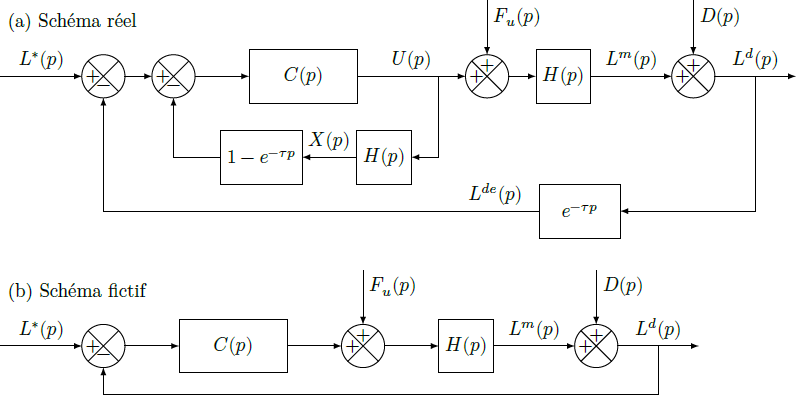
\includegraphics[width=\linewidth]{fig_12.png}
\caption{Schéma-bloc de l’asservissement en position du vérin électrique\label{fig_12}}
\end{figure}

\textbf{Notations et spécifications :}
\begin{multicols}{2}
\begin{itemize}
\item gain du capteur: $\indice{K}{capt} = \SI{588}{impulsions/m}$;
\item gain de l’ensemble réducteur et vis-écrou : $\indice{K}{red} = \SI{19.1e-6}{m/rad}$;
\item vitesse linéaire de la tige du vérin : $V(t)$ en \si{m.s^{-1}};
\item déplacement linéaire de la tige du vérin : $d(t)$ en $\si{V}$;
\item correcteur: $C_0(p)$;
\item gain du hacheur: $\indice{K}{H} = 1,163$.
\end{itemize}
\end{multicols}

Pour toute la suite du sujet, on considère : $\indice{C}{r}(p)=0$. Tout d'abord, le correcteur est consdéré unitaire $\indice{C}{0}(p)=1$.

\question{Donner l'expression littérale de la fonction de transfert en b}

\question{Donner l’expression littérale de $M(p)$ et, pour garantir un bon asservissement, l’expression 
littéralede $\indice{K}{adapt}$.}

\question{ Déterminer l’expression littérale de la fonction de transfert en boucle ouverte $\indice{G}{BO}(p)$ et mettre celle-ci sous forme canonique. Donner la classe de cette fonction de transfert. En déduire\footnote{La déduction sera (re)vue en seconde année. Il vous faudra donc sûrement la calculer.}
 la précision du système.}
 
  On donne l’expression numérique dela fonction de transfert en boucle ouverte :
  $\indice{G}{BO}(p)=\dfrac{0,0112}{p\left( 0,00028 p +1\right)}$.

\question{Tracer les diagrammes de Bode asymptotiques et réels de la fonction de transfert $\indice{G}{BO}(p)$ sur le DR3. En déduire la marge de phase de l’asservissement en effectuant toutes les constructions 
graphiques nécessaires. Conclure sur le respect de l’exigence 006 «Stabilité ».}

\begin{figure}[!h]
\centering
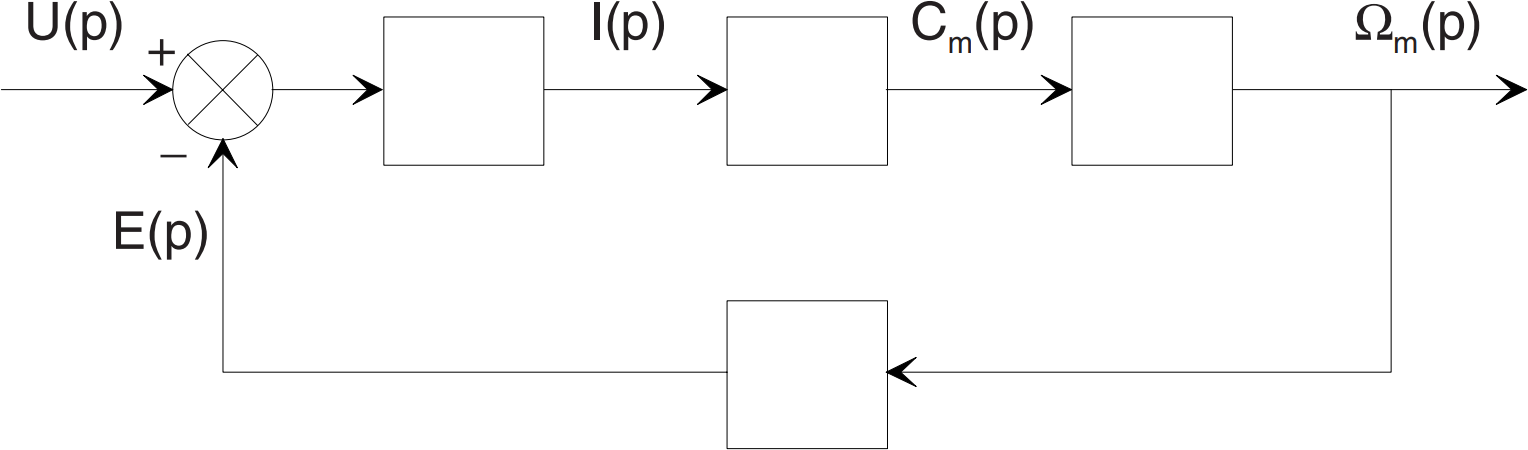
\includegraphics[width=.8\linewidth]{dr_03.png}
\caption{Diagramme de Bode \label{dr_03}}
\end{figure}

 On désire quantifier la rapidité du système à la suite d’une sollicitation en échelon. On donne les 
relations permettant de calculer le temps de réponse à 5\%, noté $\indice{t}{r5\%}$, pour un système d’ordre deux (avec $\xi$ le facteur d’amortissement et $\omega_0$ la pulsation propredu système non amorti):

$$
\left\{ 
\begin{array}{l}
\xi < \dfrac{1}{\sqrt{2}}, \indice{t}{r5\%} \simeq \dfrac{3\xi}{ \omega_0} \\
\xi > \dfrac{1}{\sqrt{2}}, \indice{t}{r5\%} \simeq \dfrac{6\xi }{\omega_0} \\
\end{array}
\right.
$$ 


\question{ Déterminer et calculer les paramètres caractéristiques de la fonction de transfert en boucle 
fermée $\indice{G}{BF}=\dfrac{D(p)}{D_c(p)}$. En déduire le temps de réponse de l’asservissement en vitesse. Conclure sur le respect de l’exigence 004 «Rapidité».}

Afin d’améliorer les performances de l’asservissement, on choisit un correcteur proportionnel de gain 
$\indice{K}{D}$ tel que $C_0(p) = \indice{K}{D}$. La valeur numérique du gain sera déterminéeà partir de deux méthodes :
\begin{itemize}
\item approche graphique, à partir de la marge de phase (maîtrise de la stabilité);
\item approche analytique, à partir d’un comportement imposé.
\end{itemize}

\question{À partir de constructions graphiques sur la figure \ref{dr_03}, donner la valeur du gain du correcteur $\indice{K}{D1}$, permettant de garantir une marge de phase supérieure à 70\degres. La valeur de $\indice{K}{D1}$ vous paraît-elle pertinente et réaliste ?}

 On impose un temps de réponse à 5\% de \SI{5}{s} et un facteur d’amortissement $\xi$ supérieur à 1.
 On donne l’expression numérique de $\indice{G}{BF}(p)$ avec un correcteur de gain $\indice{K}{D}$ :
 $\indice{G}{BF}(p)=\dfrac{1}{\dfrac{0,025}{K_D}p^2+\dfrac{89}{K_D}p +1}$.
 
 
\question{À partir des équations liant le temps de réponse, le facteur d’amortissement et la pulsation 
propre ainsi que de l’expression numérique de $\indice{G}{BF}(p)$, donner une expression liant $t_{r5\%}$  et $\indice{K}{D2}$. En déduire la valeur de $\indice{K}{D2}$ permettant de respecter la contrainte imposée en termes de rapidité.}


 On donne ci-dessous les tracés de la sortie du système asservi à la suite d’un échelon de consigne de 
\SI{10}{cm} pour $\indice{K}{D1} = \num{220000}$ et $\indice{K}{D2} = 53$.


\begin{figure}[!h]
\centering
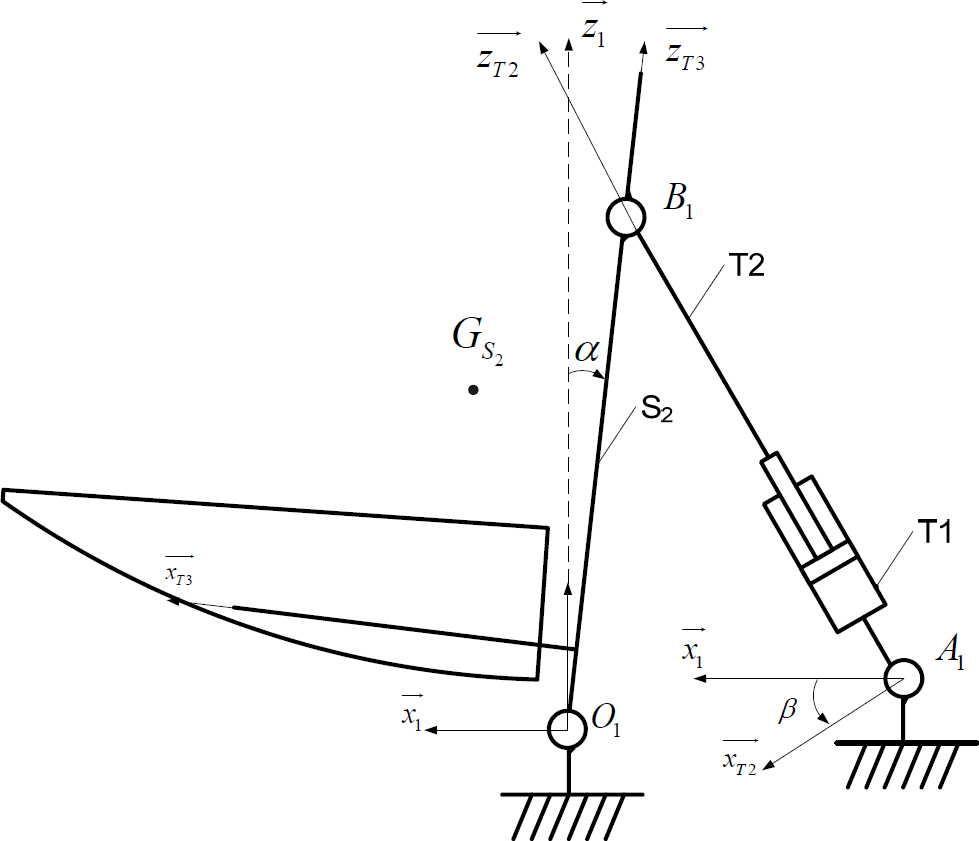
\includegraphics[width=\linewidth]{fig_13.png}
\caption{Réponses indicielles du système asservi \label{fig_13}}
\end{figure}

\question{Commenter les courbes (respect des exigences) et choisir le correcteur qui vous paraît le plus 
pertinent.}
